\documentclass{ani-intermediate}
\usepackage[colorlinks=true,
     linkcolor=CadetBlue4,
     filecolor=CadetBlue4,
     citecolor=CadetBlue4,      
     urlcolor=CadetBlue4]{hyperref}
\usepackage{rotating}

\usepackage{lipsum} % sampling purposes

\begin{document}


\frontmatter

\coverart{images/FARFETCH-logo.pdf}
\footerart{images/FUNDOS-3logos.pdf}
\reportnum{Interim Technical Scientific Report | No. }

\program{Interim Technical Scientific Report}

\title{Incentive System for Research and Technological Development (R\&D) – Projects in Co-promotion\\International Partnerships}
\subtitle{}
\date{}

\reporttype{Final Report}

%\preparedfor{}

\maketitle

\tableofcontents

\listoffiguresandtables

\mainmatter

\chapter{Identification}

\begin{table}[!htp]
  \begin{tabular}{|l|p{.5\textwidth}|}
    \hline
    Project No.:                             & \\   \hline
    Project acronym:                         & \\   \hline
    Project title:                           & \\   \hline
    Project start date:                      & \\   \hline
    Project duration:                        & \\   \hline
    Reporting period:                        & \\   \hline
    Periodic report No.:                     & \\   \hline
    Project ``Web site'' or ``microsite'':   & \\   \hline
    Consortium composition:                  & \\   \hline
  \end{tabular}
\end{table}

\chapter{Project summary and general goals}
\lipsum[1-4]

\section{Scientific and Technology Motivation for the project}
\section{Objectives}
\section{Gantt Chart}

\begin{figure}[!htp]
  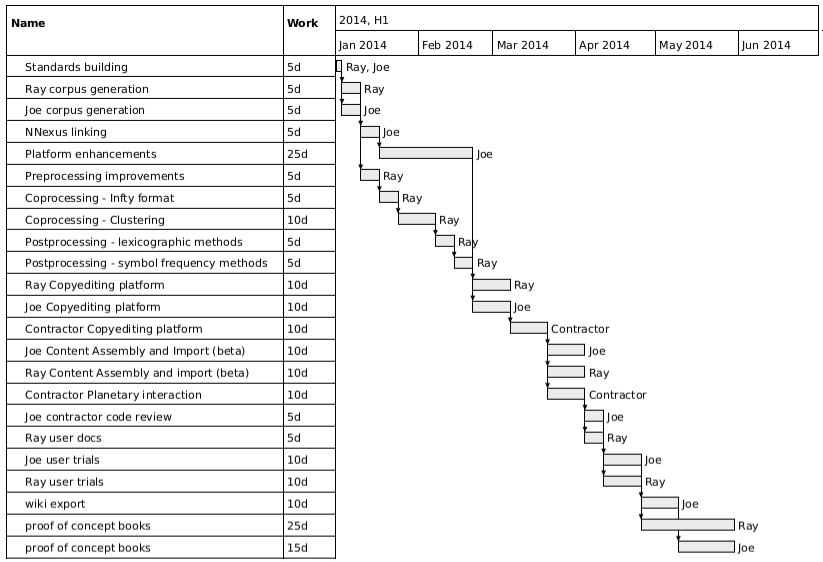
\includegraphics[width=1\textwidth]{images/gantt.png}
  \caption{A Gantt Chart (from \href{https://commons.wikimedia.org/wiki/File:Planetmathbooks_gantt.png}{wikimedia}).}
\end{figure}

\chapter{Summary of work performed}
\lipsum[5-9]


  \section{Deliverables and milestones}
  \subsection{Deliverables}
  \lipsum[10-12]

  \begin{sidewaystable}
    \center
    \scriptsize
    \begin{tabular}{|p{0.05\textwidth}|p{0.05\textwidth}|p{0.05\textwidth}|p{0.05\textwidth}|p{0.05\textwidth}|p{0.05\textwidth}|p{0.2\textwidth}|p{0.05\textwidth}|p{0.2\textwidth}|}
      \hline
      Deliverable No. & Task No. & Deliverable Title & Deliverable type & Scheduled delivery date of Annex B & Effective Delivery Date & If not delivered, why? & Disclosure Level & Comments \\ \hline
    \end{tabular}
    \caption{Deliverables.}
  \end{sidewaystable}

  \newpage
  \subsection{Milestones}
  \lipsum[10-12]

  \begin{sidewaystable}
    \center
    \scriptsize
    \begin{tabular}{|p{0.05\textwidth}|p{0.05\textwidth}|p{0.05\textwidth}|p{0.05\textwidth}|p{0.1\textwidth}|p{0.1\textwidth}|p{0.1\textwidth}|p{0.2\textwidth}|p{0.2\textwidth}|}
      \hline
      Milestone No. & Task No. & Milestone title & Verification methods & Scheduled delivery date of Annex B & Effective Delivery Date Achieved & If not achieved, why? & Comments \\ \hline
    \end{tabular}
    \caption{Milestones.}
  \end{sidewaystable}
  \newpage

\section{Potential constraints that may affect the execution of the project and proposed measures for their mitigation}
\lipsum[13-20]

\section{Promotion and dissemination of results}
\lipsum[20-24]

\begin{table}[!htp]
  \begin{tabular}{|p{0.75\textwidth}|p{0.25\textwidth}|}
    \hline
    \textbf{Typology of Action for Promotion and Dissemination of Results} & \textbf{Number of Actions} \\ \hline
    Conference organization                                          &  \\ \hline
    Workshop organization                                            &  \\ \hline
    Public demonstrations of prototypes, pilot lines                 &  \\ \hline
    Press-Release                                                    &  \\ \hline
    Non-scientific publications Scientific publications + Scientific publications co-authored with company(s) &  \\ \hline
    Participation in Trade Shows and Exhibitions                     &  \\ \hline
    Flyers                                                           &  \\ \hline
    Website                                                          &  \\ \hline
    Participation in Conferences                                     &  \\ \hline
    Participation in Workshops                                       &  \\ \hline
    Participation in Brokerage Events                                &  \\ \hline
    Others                                                           &  \\ \hline
  \end{tabular}
  \caption{Promotion and dissemination of results.}
\end{table}


\chapter{Presentation of developments obtained in the reporting period}

\section{Presentation of the results achieved by activity}
\cite{sigfridsson}\lipsum[25-30]

\section{Deviations from what was foreseen in the application, by activity}
\lipsum[30-32]

\chapter{Financial Execution}
\lipsum[33-35]



\nocite{*}
\bibliographystyle{unsrt}
\bibliography{biblatex-examples}

\end{document}
